%\chapter*{Anhang}
%\large{
%Anhang 1\par
%Anhang 2


% setzt die Bildunterschriften auf A1 (A=Anhang)
\renewcommand{\thefigure}{A\arabic{figure}} 
\chapter{Anhang}

\subsection*{Elektronischer Anhang }

\subsection*{Fahrzeugdaten}
\begin{figure}[hb!]
	\caption{Engine Power}
	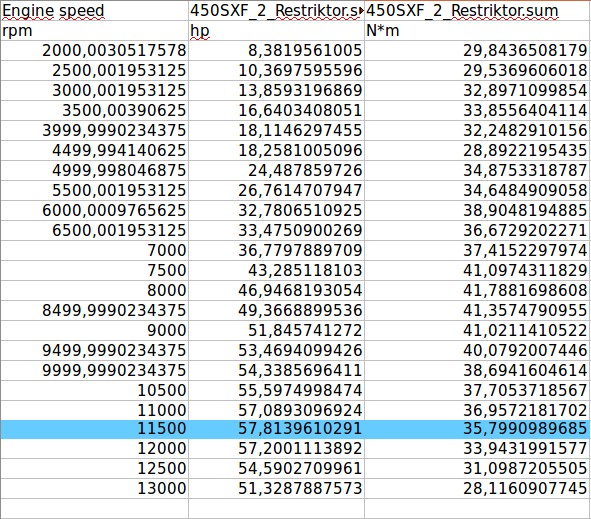
\includegraphics[width=350pt]{Abbildungen/Engine_power.png}
	\label{fig:enginePower}
\end{figure}

\begin{figure}[hb!]
	\caption{Max Tire Force}
	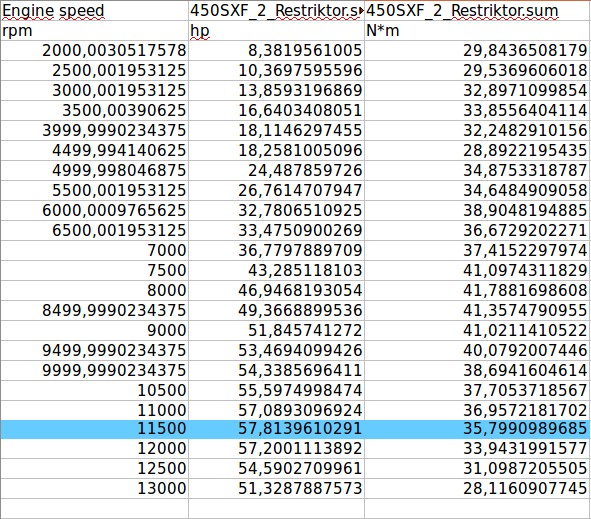
\includegraphics[width=350pt]{Abbildungen/Engine_power.png}
	\label{fig:maxTireForce}
\end{figure}



 \subsection*{Einbindung Grafik im Anhang}
  \begin{figure}[h!]
  \begin{centering}
  {
\includegraphics[width=0.33\textwidth]{Abbildungen/fau.png}}
   \caption{Unterschrift Bild x Die auf die Rotationsfrequenz des Innenzylinders normierten Eigenfrequenzen der gefun-denen Grundmoden der Taylor-Strömung für h(Die azimutale Wellenzahl ist mit m  bezeichnet.)}
  \end{centering}
  \end{figure}








